
% This LaTeX was auto-generated from MATLAB code.
% To make changes, update the MATLAB code and republish this document.

\documentclass{article}
\usepackage{graphicx}
\usepackage{color}

\sloppy
\definecolor{lightgray}{gray}{0.5}
\setlength{\parindent}{0pt}

\begin{document}

    
    

\section*{7. Convergence for differentiable functions}

\begin{verbatim}
ATAPformats
\end{verbatim}
\begin{par}
The principle mentioned at the end of the last chapter might be regarded as the central dogma of approximation theory: the smoother a function, the faster its approximants converge as $n\to\infty$.  Connections of this kind were explored in the early years of the 20th century by three of the founders of approximation theory: Charles de la $\hbox{Vall\'ee}$ Poussin (1866--1962), a mathematician at Leuven in Belgium, Sergei Bernstein (1880--1968), a Ukrainian mathematician who had studied with Hilbert in $\hbox{G\"ottingen}$, and Dunham Jackson (1888--1946), an American student of Landau's also at $\hbox{G\"ottingen}$. (Henri Lebesgue in France (1875--1941) also proved some of the early results. For remarks on the history see [Goncharov 2000] and [Steffens 2006].) Bernstein made the following comment concerning best approximation errors $E_n(f) = \|f-p_n^*\|_\infty$ (see Chapter 10) in his summary article for the International Congress of Mathematicians in 1912 [Bernstein 1912a]:
\end{par} \vspace{1em}
\begin{par}
 \em
The general fact that emerges from this study is the existence of a most
intimate connection between the differential properties of the function
$f(x)$ and the asymptotic rate of decrease of the positive numbers
$E_n[f(x)]$.\footnote{``Le fait g\'en\'eral qui se d\'egage de cette
\'etude est l'existence d'une liaison des plus intimes entre les
propri\'et\'es diff\'erentielles de la fonction $f(x)$ et la loi
asymptotique de la d\'ecroissance des nombres positifs $E_n[f(x)]$.''}

\end{par} \vspace{1em}
\begin{par}
In this and the next chapter our aim is to make the smoothness--approximability link precise in the context of Chebyshev projections and interpolants. Everything here is analogous to results for Fourier analysis of periodic functions, and indeed, the whole theory of Chebyshev interpolation can be regarded as a transplant to nonperiodic functions on $[-1,1]$ of the theory of trigonometric interpolation of periodic functions on $[-\pi,\pi]$.
\end{par} \vspace{1em}
\begin{par}
Suppose a function $f$ is $\nu$ times differentiable on $[-1,1]$, possibly with jumps in the $\nu\kern .7pt\hbox{th}$ derivative, and suppose you look at the convergence of its Chebyshev interpolants as $n\to\infty$, measuring the error in the $\infty$-norm. You will typically see convergence at the rate $O(n^{-\nu})$.  We can explore this effect readily with Chebfun.  For example, the function $f(x) = |x|$ is once differentiable with a jump in the first derivative at $x=0$, and the convergence curve nicely matches $n^{-1}$ (shown as a straight line). Actually the match is more than just nice in this case---it is exact, with $p_n$ taking its maximal error at the value $p(0) = 1/n$ for odd $n$.  (For even $n$ the error is somewhat smaller.)
\end{par} \vspace{1em}
\begin{par}
 \vskip -2em 
\end{par} \vspace{1em}
\begin{verbatim}
x = chebfun('x'); f = abs(x);
nn = 2*round(2.^(0:.3:7))-1;
ee = 0*nn;
for j = 1:length(nn)
    n = nn(j); fn = chebfun(f,n+1); ee(j) = norm(f-fn,inf);
end
hold off, loglog(nn,1./nn,'r'), FS = 'fontsize';
text(5,0.07,'n^{-1}',FS,12)
grid on, axis([1 300 1e-3 2])
hold on, loglog(nn,ee,'.')
title('Linear convergence for a differentiable function',FS,9)
\end{verbatim}

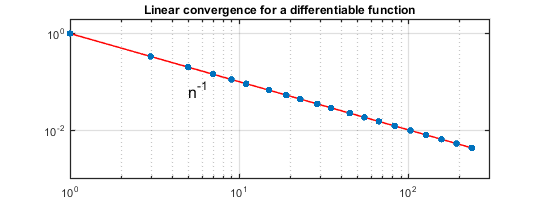
\includegraphics [width=4in]{chap7_01.png}
\begin{par}
 \vskip 1pt 
\end{par} \vspace{1em}
\begin{par}
Similarly, we get cubic convergence for $$ f(x) = |\sin(5x)|^3 , \eqno (7.1) $$ which is three times differentiable with jumps in the third derivative at $x=0$ and $\pm \pi/5$.
\end{par} \vspace{1em}
\begin{par}
 \vskip -2em 
\end{par} \vspace{1em}
\begin{verbatim}
f = abs(sin(5*x)).^3;
for j = 1:length(nn)
    n = nn(j); fn = chebfun(f,n+1); ee(j) = norm(f-fn,inf);
end
hold off, loglog(nn,nn.^-3,'r')
text(4,.0015,'n^{-3}',FS,12)
grid on, axis([1 300 2e-6 10])
hold on, loglog(nn,ee,'.')
title('Cubic convergence for a 3-times differentiable function',FS,9)
\end{verbatim}

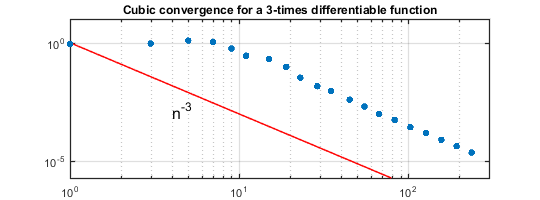
\includegraphics [width=4in]{chap7_02.png}
\begin{par}
 \vskip 1pt 
\end{par} \vspace{1em}
\begin{par}
Encouraged by such experiments, you might look in a book to try to find theorems about $O(n^{-\nu})$.  If you do, you'll run into two difficulties.  First, it's hard to find theorems about Chebyshev interpolants, for most of the literature is about other approximations such as best approximations (see Chapters 10 and 16) or interpolants in Chebyshev polynomial roots rather than extrema. Second, you will probably fall one power of $n$ short!  In particular, the most commonly quoted of the \textit{Jackson theorems} asserts that if $f$ is $\nu$ times \textit{continuously} differentiable on $[-1,1]$, then its best polynomial approximations converge at the rate $O(n^{-\nu})$ [Jackson 1911; Cheney 1966, $\hbox{sec.~4.6}$]. But the first and third derivatives of the functions we just looked at, respectively, are not continuous. Thus we must settle for the zeroth and second derivatives, respectively, if we insist on continuity, so this theorem would ensure only $O(n^0)$ and $O(n^{-2})$ convergence, not the $O(n^{-1})$ and $O(n^{-3})$ that are actually observed.  And it would apply to best approximations, not Chebyshev interpolants.
\end{par} \vspace{1em}
\begin{par}
We can get the result we want by recognizing that most functions encountered in applications have a property that is not assumed in the theorems just mentioned: \textit{bounded variation}.  A function, whether continuous or not, has bounded variation if its total variation is finite.  The \textit{total variation} is the 1-norm of the derivative (as defined if necessary in the distributional sense; see [Ziemer 1989, $\hbox{chap.~5}$] or [Evans \& Gariepy 1991, $\hbox{sec.~5.10}$]).  We can compute this number conveniently with Chebfun by writing a function called \texttt{tv} that evaluates $\|f'\|_1$ for a given function $f$:
\end{par} \vspace{1em}
\begin{par}
 \vskip -2em 
\end{par} \vspace{1em}
\begin{verbatim}
tv = @(f) norm(diff(f),1);
\end{verbatim}
\begin{par}
Here are the total variations of $x$ and $\sin(10\pi x)$ over $[-1,1]$:
\end{par} \vspace{1em}
\begin{par}
 \vskip -2em 
\end{par} \vspace{1em}
\begin{verbatim}
disp([tv(x) tv(sin(10*pi*x))])
\end{verbatim}

        \color{lightgray} \begin{verbatim}   2.000000000000000  40.000000000000007
\end{verbatim} \color{black}
    \begin{par}
Here is the total variation of the derivative of $|x|$:
\end{par} \vspace{1em}
\begin{par}
 \vskip -2em 
\end{par} \vspace{1em}
\begin{verbatim}
tv(diff(abs(x)))
\end{verbatim}

        \color{lightgray} \begin{verbatim}ans =
     2
\end{verbatim} \color{black}
    \begin{par}
Here is the total variation of the third derivative of the function $f$ of (7.1):
\end{par} \vspace{1em}
\begin{par}
 \vskip -2em 
\end{par} \vspace{1em}
\begin{verbatim}
tv(diff(f,3))
\end{verbatim}

        \color{lightgray} \begin{verbatim}ans =
     2.102783663434700e+04
\end{verbatim} \color{black}
    \begin{par}
It is the finiteness of this number that allowed the Chebyshev interpolants to this function $f$ to converge as fast as $O(n^{-3})$.
\end{par} \vspace{1em}
\begin{par}

To get to a precise theorem, we begin with a bound on Chebyshev
coefficients, an improvement (in the definition of the quantity $V$) of a
similar result in [Trefethen 2008] whose proof was provided
by Endre S\"uli. The condition of {\em absolute
continuity} is a standard one which we shall not make detailed use of, so
we will not discuss.  An absolutely continuous function is equal to the
integral of its derivative, which exists almost everywhere and is
Lebesgue integrable.

\end{par} \vspace{1em}
\begin{par}
 \em
{\bf Theorem 7.1. Chebyshev coefficients of differentiable functions.}
For an integer $\nu \ge 0$, let $f$ and its derivatives through
$f^{(\nu -1)}$ be absolutely continuous on $[-1,1]$ and suppose the
$\nu$th derivative $f^{(\nu )}$ is of bounded variation $V$.  Then for $k\ge
\nu +1$, the Chebyshev coefficients of $f$ satisfy
$$ | a_k | \le  {2V\over \pi k(k-1)\cdots (k-\nu )}
\le {2V\over \pi (k-\nu )^{\nu +1}}.  \eqno (7.2) $$
\vspace{-1em} 
\end{par} \vspace{1em}
\begin{par}
\textit{Proof.} As in the proof of Theorem 3.1, setting $x = {\textstyle{1\over 2}}(z+z^{-1})$ with $z$ on the unit circle gives $$ a_k={1\over\pi i}\int_{|z|=1}f({\textstyle{1\over 2}}(z+z^{-1}))\, z^{k-1}\,dz, $$ and integrating by parts with respect to $z$ converts this to $$ a_k={-1\over\pi i}\int_{|z|=1}f'({\textstyle{1\over 2}}(z+z^{-1}))\, {z^k\over k}\,{dx\over dz}\,dz\,; \eqno (7.3) $$ the factor $dx/dz$ appears since $f'$ denotes the derivative with respect to $x$ rather than $z$. Suppose now $\nu =0$, so that all we are assuming about $f$ is that it is of bounded variation $V = \|f'\|_1$. Then we note that this integral over the upper half of the unit circle is equivalent to an integral in $x\kern 1pt$; the integral over the lower half gives another such integral.  Combining the two gives $$ a_k={1\over\pi i}\int_{-1}^1 f'(x)\, {z^k - z^{-k}\over k}\,dx ={2\over\pi}\int_{-1}^1 f'(x)\, \hbox{Im}\, {z^k \over k}\,dx, $$ and since $|z^k/k| \le 1/k$ for $x\in[-1,1]$ and $V = \|f'\|_1$, this implies $|a_k| \le 2V/\pi k$, as claimed.
\end{par} \vspace{1em}
\begin{par}
If $\nu >0$, we replace $dx/dz$ by ${\textstyle{1\over 2}}(1-z^{-2})$ in (7.3), obtaining $$ a_k= - {1\over\pi i}\int_{|z|=1}f'({\textstyle{1\over 2}}(z+z^{-1}))\, \left[{z^k\over 2k}-{z^{k-2}\over 2k}\right]\,dz . $$ Integrating by parts again with respect to $z$ converts this to $$ a_k={1\over\pi i}\int_{|z|=1}f''({\textstyle{1\over 2}}(z+z^{-1}))\, \left[{z^{k+1}\over 2k(k+1)}-{z^{k-1}\over 2k(k-1)}\right]\,{dx\over dz}\,dz. $$ Suppose now $\nu =1$ so that we are assuming $f'$ has bounded variation $V = \|f''\|_1$. Then again this integral is equivalent to an integral in $x$, $$ a_k={-2\over\pi}\int_{-1}^1 f''(x)\, \hbox{Im} \left[{z^{k+1}\over 2k(k+1)}-{z^{k-1}\over 2k(k-1)}\right]\,dx. $$ Since the term in square brackets is bounded by $1/k(k-1)$ for $x\in[-1,1]$ and $V = \|f'' \|_1$, this implies $|a_k| \le 2V/\pi k(k-1)$, as claimed.
\end{par} \vspace{1em}
\begin{par}
If $\nu >1$, we continue in this fashion with a total of $\nu +1$ integrations by parts with respect to $z$, in each case first replacing $dx/dz$ by ${\textstyle{1\over 2}}(1-z^{-2})$. At the next step the term that appears in square brackets is $$ \left[{z^{k+2}\over 4k(k+1)(k+2)} - {z^k \over 4k^2(k+1)} - {z^k\over 4k^2(k-1)} +{z^{k-2}\over 4k(k-1)(k-2)}\right], $$ which is bounded by $1/k(k-1)(k-2)$ for $x\in[-1,1]$.  And so on. $~\hbox{\vrule width 2.5pt depth 2.5 pt height 3.5 pt}$
\end{par} \vspace{1em}
\begin{par}
From Theorems 3.1 and 7.1 we can derive consequences about the accuracy of Chebyshev projections and interpolants. Variations on the estimate (7.5) can be found as Corollary 2 of [Mastroianni \& Szabados 1995] and Theorem 2 of [Mastroianni \& Russo 2010]. The analogous result for best approximations as opposed to Chebyshev interpolants or projections was announced in [Bernstein 1911] and proved in [Bernstein 1912b].
\end{par} \vspace{1em}
\begin{par}
 \em
{\bf Theorem 7.2. Convergence for differentiable functions.}
If $f$ satisfies the conditions of Theorem $7.1$, with $V\kern -.7pt $
again denoting the total variation of $f^{(\nu)}$ for some $\nu\ge 1$,
then for any $n>\nu$, its Chebyshev projections satisfy
$$ \|f-f_n\| \le {2V\over \pi \nu  (n-\nu )^\nu } \eqno (7.4) $$
and its Chebyshev interpolants satisfy
$$ \|f-p_n\| \le {4V\over \pi \nu  (n-\nu )^\nu }. \eqno (7.5) $$
\vspace{-1em} 
\end{par} \vspace{1em}
\begin{par}
\textit{Proof.}  For (7.4), Theorem 7.1 applied to equation (4.8) gives us $$ \|f-f_n\| \,\le \sum_{k=n+1}^\infty |a_k| \,\le {2V\over\pi} \sum_{k=n+1}^\infty (\kern 1pt k-\nu )^{-\nu -1} $$ and this sum can in turn be bounded by $$ \int_n^\infty (s-\nu )^{-\nu -1} ds = {1\over \nu  (n-\nu )^\nu }. $$ For (7.5), we use (4.9) instead of (4.8) and get the same bound except with coefficients $2|a_k|$ rather than $|a_k|$. $~\hbox{\vrule width 2.5pt depth 2.5 pt height 3.5 pt}$
\end{par} \vspace{1em}
\begin{par}
In a nutshell: a $\nu\kern -2.5 pt $ th derivative of bounded variation implies convergence at the algebraic rate $O(n^{-\nu})$.  Here is a way to remember this message. Suppose we try to approximate the step function $\hbox{sign}(x)$ by polynomials.  There is no hope of convergence, since polynomials are continuous and $\hbox{sign}(x)$ is not, so all we can achieve is accuracy $O(1)$ as $n\to\infty$.  That's the case $\nu =0$. But now, each time we make the function ``one derivative smoother,'' $\nu$ increases by 1 and so does the order of convergence.
\end{par} \vspace{1em}
\begin{par}
How sharp is Theorem 7.2 for our example functions?  In the case of $f(x) = |x|$, with $\nu =1$ and $V=2$, it predicts $\|f-f_n\| \le 4/\pi(n-1)$ and $\|f-p_n\| \le 8/\pi(n-1) \approx 2.55/(n-1)$.  As mentioned above, the actual value for Chebyshev interpolation is $\|f-p_n\| = 1/n$ for odd $n$. The minimal possible error in polynomial approximation, with $p_n$ replaced by the best approximation $p_n^*$ (Chapter 10), is $\|f-p_n^*\| \sim 0.280169\dots n^{-1}$ as $n\to\infty$ [Varga \& Carpenter 1985]. So we see that the range from best approximant, to Chebyshev interpolant, to bound on Chebyshev interpolant is less than a factor of 10.  The approximation of $|x|$ was a central problem studied by Lebesgue, de la $\hbox{Vall\'ee}$ Poussin, Bernstein, and Jackson a century ago, and we shall consider it further in Chapter 25.
\end{par} \vspace{1em}
\begin{par}
The results are similar for the other example, $f(x) = |\sin(5x)|^3$, whose third derivative, we saw, has variation $V \approx 16528$. Equation (7.5) implies that the Chebyshev interpolants satisfy $\|f-p_n\| < 7020/(n-1)^3$, whereas in fact, we have $\|f-p_n\| \approx 309/n^3$ for large odd $n$ and $\|f-p_n^*\| \approx 80/n^3$.
\end{par} \vspace{1em}
\begin{par}
We close with a comment about Theorem 7.2. We have assumed in this theorem that $f^{(\nu)}$ is of bounded variation.  A similar but weaker condition would be that $f^{(\nu-1)}$ is Lipschitz continuous (Exercise 7.2). This weaker assumption is enough to ensure $\|f-p_n^*\| = O(n^{-\nu})$ for the best approximations $\{p_n^*\}$; this is one of the Jackson theorems. On the other hand it is not enough to ensure $O(n^{-\nu})$ convergence of Chebyshev projections and interpolants.  The reason we emphasize the stronger implication with the stronger conclusion is that in practice, one rarely deals with a function that is Lipschitz continuous while lacking a derivative of bounded variation, whereas one constantly deals with projections and interpolants rather than best approximations.
\end{par} \vspace{1em}
\begin{par}
Incidentally, it was de la $\hbox{Vall\'ee}$ Poussin [1908] who first showed that the strong hypothesis is enough to reach the weak conclusion: if $f^{(\nu)}$ is of bounded variation, then $\|f-p_n^*\| = O(n^{-\nu})$ for the best approximation $p_n^*$. Three years later Jackson [1911] sharpened the result by weakening the hypothesis as just indicated.
\end{par} \vspace{1em}
\begin{par}

\begin{displaymath}
\framebox[4.7in][c]{\parbox{4.5in}{\vspace{2pt}\sl
{\sc Summary of Chapter 7.}
The smoother a function $f$ defined on $[-1,1]$ is, the faster its
approximants converge.  In particular, if the $\nu$th derivative of $f$
is of bounded variation $V$, then the Chebyshev coefficients $\{a_k\}$ of
$f$ satisfy $|a_k| \le 2\pi^{-1}V(k-\nu)^{-\nu-1}$.  For $\nu\ge 1$, it
follows that the degree~$n$ Chebyshev projection and interpolant of $f$
both have accuracy $O(V n^{-\nu})$.\vspace{2pt}}}
\end{displaymath}

\end{par} \vspace{1em}
\begin{par}
 \smallskip\small\parskip=2pt
{\bf Exercise 7.1.  Total variation.}  (a) Determine numerically the
total variation of $f(x) = \sin(100 x)/(1+x^2)$ on $[-1,1]$.  (b) It is
no coincidence that the answer is close to $100$, and indeed the total
variation of $\sin(Mx)/(1+x^2)$ on $[-1,1]$ is asymptotic to $M$ as
$M\to\infty$. Explain why.
\par
{\bf Exercise 7.2.  Lipschitz continuous $\hbox{vs.}$ derivative of
bounded variation.} (a) Prove that if the derivative $f'$ of a function
$f$ has bounded variation, then $f$ is Lipschitz continuous.  (b) Give an
example to show that the converse does not hold.
\par
{\bf Exercise 7.3.  Convergence for Weierstrass's function.}
Exercise 6.1 considered a ``pathological function of Weierstrass''
$w(x)$ that is continuous but nowhere differentiable on $[-1,1]$.
(a) Make an anonymous function in Matlab that evaluates $w({\tt xx})$ for
a vector ${\tt xx}$ to machine precision by taking the sum to 53 terms.
(b) Use Chebfun to produce a plot of $\|w-p_n\|$ accurate enough and for
high enough values of $n$ to confirm that convergence appears to take
place as $n\to\infty$. Thus $w$ is not one of the functions for which
interpolants fail to converge, a fact we can prove with the
techniques of Chapter 15 (Exercise 15.9).
\par
{\bf Exercise 7.4.  Sharpness of Theorem 7.2.}  Consider the functions
(a) $f(x) = |x|$, (b) $f(x) = |x|^5$, (c) $f(x) = \sin(100x)$. In each
case  plot, as functions of $n$, the error $\|f-p_n\|$ in Chebyshev
interpolation on $[-1,1]$ and the bound on this quantity from (7.5).  How
close is the bound to the actuality?  In cases (a) and (b) take $\nu$ as large as
possible, and in case (c), take $\nu = 2$, $4$, and $8$.
\par
{\bf Exercise 7.5.  Total variation.}  Let $f$ be a smooth function defined
on $[0,1]$ and let $t(x)$ be its total variation over the interval
$[0,x]$.  What is the total variation of $t$ over $[0,1]$?
\par
{\bf Exercise 7.6.  Chebyshev coefficients of a spline.}  A cubic spline is a piecewise
cubic polynomial with two continuous derivatives.
(a) How fast must the Chebyshev series coefficients of a cubic spline decay?
(b) Test this prediction with the Chebfun commands
\verb|f=chebfun('exp(x)')|, \verb|s=spline(linspace(-1,1,10),f)|,
\verb|p=chebfun(s)|, \verb|chebpolyplot(p,'loglog')|.
\par 
\end{par} \vspace{1em}



\end{document}
    
